\documentclass{beamer}

\usepackage[utf8]{inputenc}
\usetheme{Madrid}

\title[Loss Landscape Convergence]{Neural Networks Loss Landscape Convergence in Different Low-Dimensional Spaces}
\author{Tem Nikitin \ Nikita Kiselev}
\institute[MIPT]{Moscow Institute of Physics and Technology}
\date{\today}

\begin{document}

\begin{frame}
    \titlepage
\end{frame}

\begin{frame}{Problem Statement}
    \begin{itemize}
        \item Neural networks achieve higher accuracy with larger datasets.
        \item However, computational resources limit training possibilities.
        \item Key question: \textbf{When does additional data stop reshaping the loss landscape?}
    \end{itemize}
\end{frame}

\begin{frame}{Proposed Method}
    \begin{itemize}
        \item Analyze loss landscape via Hessian eigenvectors.
        \item Project high-dimensional parameter space onto lower-dimensional space.
        \item Utilize Monte-Carlo methods to approximate landscape changes.
    \end{itemize}
\end{frame}

\begin{frame}{Main Idea}
    \begin{itemize}
        \item \textbf{Hessian-based projections} identify primary curvature directions.
        \item Calculate a $\Delta$-function to quantify changes when increasing dataset size:
              $$\Delta_k = \int (L_k(w)-L_{k-1}(w))^2 p(w) dw$$
        \item Identify the threshold at which further data does not significantly alter landscape.
    \end{itemize}
\end{frame}

% Слайд из файла пользователя (обязательный)
\begin{frame}{Neural Networks Loss Landscape Convergence in Different Low-Dimensional Spaces}

    \textbf{Goal:} Measure how the loss function changes as the training set size grows:
    \[
        \Delta_k = \mathbb{E}_{p(\mathbf{w})}\Bigl(\mathcal{L}_{k}(\mathbf{w}) - \mathcal{L}_{k-1}(\mathbf{w})\Bigr)^2.
    \]

    \textbf{Method:}
    \begin{itemize}
        \item \textbf{Monte Carlo:} Generate points near the minimum according to $p(\mathbf{w})$ and average the differences.
        \item \textbf{Hessian Eigenvectors:} Use directions with the largest eigenvalues to focus on key curvature components.
    \end{itemize}

    \begin{columns}[t]
        \column{0.35\textwidth}
        \centering
        \hspace*{-2cm}
        \includegraphics[width=0.70\textwidth]{img/LS_16.jpg}\\

        \column{0.47\textwidth}
        \centering
        \vspace*{-3cm}
        \hspace*{-2.2cm}
        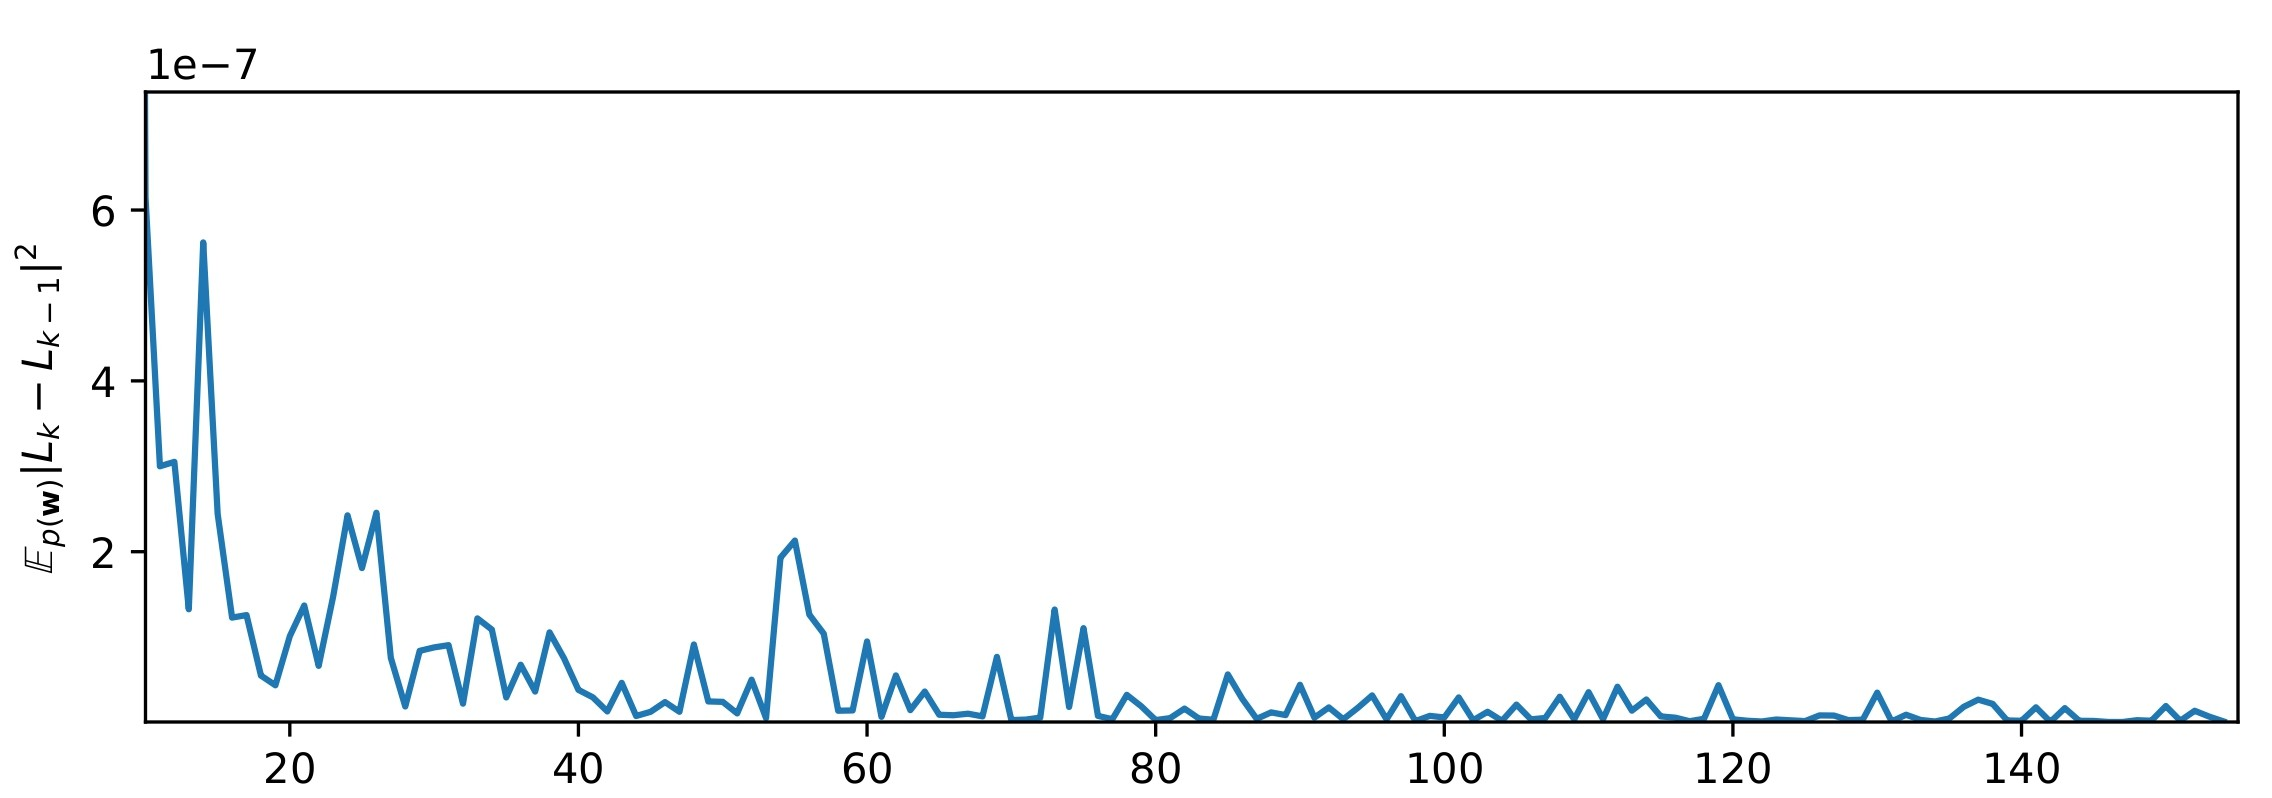
\includegraphics[width=1.375\textwidth]{img/D_32.jpg}\\
        \hspace*{-1.2cm}
        \scriptsize \textit{$\Delta_k$ function}
    \end{columns}

\end{frame}

\begin{frame}{Experiment Results}
    \begin{itemize}
        \item Experiments conducted on MNIST and Fashion-MNIST datasets.
        \item Low-dimensional visualization clearly illustrates stabilization.
        \item Verified theoretical bounds empirically.
    \end{itemize}
\end{frame}

\begin{frame}{Practical Implications}
    \begin{itemize}
        \item Enables identification of minimal viable dataset size.
        \item Reduces computational cost significantly.
        \item Provides guidelines for efficient data collection.
    \end{itemize}
\end{frame}

\begin{frame}{References}
    \scriptsize
    \begin{thebibliography}{9}
        \bibitem{1} Soydaner, D. \textit{Optimization algorithms for deep learning}, 2020.
        \bibitem{2} Wu et al. \textit{Loss landscape and generalization}, 2017.
        \bibitem{3} Petersen, Pedersen. \textit{The matrix cookbook}, 2012.
        \bibitem{4} Deng, L. \textit{MNIST database}, 2012.
        \bibitem{5} Xiao et al. \textit{Fashion-MNIST}, 2017.
        \bibitem{6} Kiselev, Grabovoy. \textit{Unraveling the Hessian}, 2024.
        \bibitem{7} Sagun et al. \textit{Hessian analysis of networks}, 2018.
    \end{thebibliography}
\end{frame}

\end{document}
